\section{Experiments}
\label{sec:experiment}
To measure the efficacy of the TSVD, we have considered three different categories of projects and run our TSVD on those dataset. Afterwards, we record the number of bugs our TSVD can detect and the overhead it's needed. We also compare our results with the existing concurrency bug detection technique namely RV-Predict. The details of each work is in the following sections.

\subsection{Experimental Settings}
We run our experiments on Ubuntu 20.04.2 LTS operating system. We run all our benchmark suite on a server machine with Intel(R) Core(TM)
i9-9900 CPU @ 3.10GHz. The architecture is x86\_64 and it has 16 CPUs.

\subsection{DataSet Description}
To run the experiments, we have considered a total 31 projects. All these projects are Java projects that build with
Maven \cite{maven} and use JUnit.
We collected the projects from three different sources as shown in Table~\ref{table:dataset} and those are 1) Toy
projects, 2) JACONTEBE projects (especially developed for concurrency bugs) and
3) open source Github thread based projects. The Toy projects are
developed by the authors of the report.

As for our evaluation, we use the JACONTEBE (Java Concurrency Test Benchmark) suite
which provides code and tests to reproduce concurrency bugs in several open
source Java projects. The bugs cover various kinds of concurrency bug types,
including atomicity violation, data race and deadlock. All these bugs the JACONTEBE can expose are real world and collected from the
projects' online bug-tracking systems. They provide the corresponding binary
.jar files for the target project. These target projects contain \textit{Apache
Commons DBCP}, \textit{Apache Derby} and \textit{Groovy}, etc. Mostly,
reproducing the bug can just use the unmodified project's binary jar files.
However, the buggy interleaving is rather infrequent and thus the JACONTEBE
dataset provides modified .jar files, in which it adds more control for
interleavings during class-loading. All the test projects are organized as an
Eclipse project, thus we can just use "\textit{java -cp}" to put our
instrumented binary .jar to incorporate our tool. The scripts to run all these
tests will be modified according to these manually written tests.


Besides this data set, we have collected 21 popular Java open source Github
projects which are maven projects and have thread instances. To get these projects, we searched on Github with some keywords such as \textit{"data
race"}, \textit{"concurrency"} and \textit{"thread"}. We determine the popularity of Github projects using the number of stars. Table \ref{table:dataset}
illustrates our considered 21 projects.

Table~\ref{table:dataset} refers to the total $31$ Java projects of these three
categories with the Line of Code (LOC) and number of tests (\#Test).


%\shanto{Position For Dataset Table}

\begin{table*}
	\centering
	\caption{the initial dataset}
	\label{table:dataset}

	\begin{tabular}{|r|l|l|r|r|}
		\hline
		\textbf{Id} & \textbf{Project Category}   & \textbf{Project Name}                                                                       & \textbf{Line of Code} & \textbf{\#Tests} \\ \hline
		1           & \multirow{2}{*}{toy project} & Data-Race                                                                                    & 85                      & 1                       \\ \cline{1-1} \cline{3-5} 
		2           &                              & DataRace-Toy-Project2                                                                        & 98                      & 1                       \\ \hline
		3           & \multirow{7}{*}{JaConTeBe}   & Apache Log4j (log4j)                                                                         & 553                     & 5                       \\ \cline{1-1} \cline{3-5} 
		4           &                              & Apache Dbcp (dbcp)                                                                           & 16145                   & 4                       \\ \cline{1-1} \cline{3-5} 
		5           &                              & Apache Derby (derby)                                                                         & 1245                    & 5                       \\ \cline{1-1} \cline{3-5} 
		6           &                              & Apache Groovy (groovy)                                                                       & 1237                    & 6                       \\ \cline{1-1} \cline{3-5} 
		7           &                              & OpenJdk (jdk-6, jdk-7)                                                                       & 5231                    & 20                      \\ \cline{1-1} \cline{3-5} 
		8           &                              & Apache Lucene (lucene)                                                                       & 1879                    & 2                       \\ \cline{1-1} \cline{3-5} 
		9           &                              & Apache Pool (pool)                                                                           & 1108                    & 5                       \\ \hline
		10          & \multirow{22}{*}{github}     & Java-WebSocket                                                                               & 26092                   & 528                     \\ \cline{1-1} \cline{3-5} 
		11          &                              & macrozheng/mall                                                                              & 132034                  & 9                       \\ \cline{1-1} \cline{3-5} 
		12          &                              & google/guava                                                                                 & 363995                  & 1713746                 \\ \cline{1-1} \cline{3-5} 
		13          &                              & eugenp/tutorials                                                                             & 929619                  & 13993                   \\ \cline{1-1} \cline{3-5} 
		14          &                              & apolloconfig/apollo                                                                          & 104010                  & 901                     \\ \cline{1-1} \cline{3-5} 
		15          &                              & alibaba/druid                                                                                & 406399                  & 206                     \\ \cline{1-1} \cline{3-5} 
		16          &                              & alibaba/fastjson                                                                             & 208646                  & 273                     \\ \cline{1-1} \cline{3-5} 
		17          &                              & xkcoding/spring-boot-demo                                                                    & 44107                   & 184                     \\ \cline{1-1} \cline{3-5} 
		18          &                              & alibaba/easyexcel                                                                            & 26790                   & 277                     \\ \cline{1-1} \cline{3-5} 
		19          &                              & alibaba/canal                                                                                & 108165                  & 283                     \\ \cline{1-1} \cline{3-5} 
		20          &                              & seata/seata                                                                                  & 200915                  & 982                     \\ \cline{1-1} \cline{3-5} 
		21          &                              & xuxueli/xxl-job                                                                              & 37834                   & 20                      \\ \cline{1-1} \cline{3-5} 
		22          &                              & jenkinsci/jenkins                                                                            & 326847                  & 3206                    \\ \cline{1-1} \cline{3-5} 
		23          &                              & alibaba/Sentinel                                                                             & 83454                   & 531                     \\ \cline{1-1} \cline{3-5} 
		24          &                              & elunez/eladmin                                                                               & 14386                   & 15                      \\ \cline{1-1} \cline{3-5} 
		25          &                              & linlinjava/litemall                                                                          & 150342                  & 51                      \\ \cline{1-1} \cline{3-5} 
		26          &                              & \begin{tabular}[c]{@{}r@{}}EnterpriseQualityCoding/\\ FizzBuzzEnterpriseEdition\end{tabular} & 1740                    & 1                       \\ \cline{1-1} \cline{3-5} 
			27          &                              & openzipkin/zipkin                                                                            & 112637                  & 1268                    \\ \cline{1-1} \cline{3-5} 
			28          &                              & apache/shardingsphere                                                                        & 375926                  & 4808                    \\ \cline{1-1} \cline{3-5} 
			29          &                              & \begin{tabular}[c]{@{}r@{}}JeffLi1993/\\ springboot-learning-example\end{tabular}            & 6463                    & 36                      \\ \cline{1-1} \cline{3-5} 
				30          &                              & eclipse-vertx/vert.x                                                                         & 152153                  & 3327                    \\ \cline{1-1} \cline{3-5} 
				31          &                              & YunaiV/SpringBoot-Labs                                                                       & 65510                   & 296                     \\ \hline
	\end{tabular}

\end{table*}


\subsection{Research Questions}
To measure the effectiveness of our TSVD, we have addressed three main research questions and those are as follows.
\begin{itemize}
		        \item RQ1:  How many thread safety violations can our tool expose?
				        \item RQ2:  What is the overhead when running TSVD for the subject projects?
						        \item RQ3:  What is the effectiveness of TSVD compared to the existing techniques?
								%       \item RQ4:  What are the race characteristics of the found bugs?
								%       \item RQ4: After conducting parameter-sensitivity experiments, which combination of parameters can best balance bug exposing capability, accuracy, and cost? - (Not Answered yet)
\end{itemize}
The reason for RQ1 is to understand how effective the TSVD is by measuring the
number of detected concurrency bugs.  RQ2 is important because it indicates the
time consumption required to run TSVD on each of the projects. RQ3 is needed
because it makes a comparison between the TSVD and an existing technique to
detect concurrency bugs.  In addition to this, we will also measure the number of true positive and false positive bugs detected by our technique.

\subsubsection{RQ1: How many thread safety violations our tool can expose?}
\label{sec:eval:rq1}

To answer this question, we run TSVD on these 31 Java projects and record the
number of bugs that happened due to the thread interleavings.  Table~\ref{table:bugs} shows
the number of bugs and the location (i.e, class name and line number) of the conflicting statements. In addition
to this, we also record the number of runs needed to generate the bugs. Because
sometimes we need to run the TSVD for more than 1 time to reproduce the actual bug.
From this table, we can mention that our TSVD performance is promising in the case of both Toy
projects and JACONTEBE benchmark as both projects have concurrency bugs.
However, for the 21 open source Github projects, TSVD can identify data-race
bugs for three different projects. One possible reason not to detect data-race on those projects may be that those projects
are race free.




%\shanto{put the table for bugs found}

\begin{table*}
	\centering
	\caption{found bugs}
	\label{table:bugs}
	\resizebox{\textwidth}{!}{
			\begin{tabular}{|l|l|r|r|r|}
				\hline
				\multicolumn{1}{|c|}{\textbf{Project Name}} & \multicolumn{1}{c|}{\textbf{Conflicting Location}}     & \multicolumn{1}{c|}{\textbf{\#Bugs}} & \multicolumn{1}{c|}{\textbf{\#Lines}} & \multicolumn{1}{c|}{\textbf{\#Runs}} \\ \hline
				DataRace1                                   & dataRace/DataRace                                                      & 1                                    & \{14,27\}                               & 1                                    \\ \hline
				DataRace2                                   & …                                                      & 1                                    & \{...\}                               & 1                                    \\ \hline
				Apache Log4j (log4j)                        & org/apache/log4j/helpers/AppenderAttachableImpl        & 2                                    & \{143, 143\}                          & 3                                    \\ \hline
				Apache Log4j (log4j)                        &  org/apache/log4j/spi/ThrowableInformation                                                      & 3                                    & \{93, 90\}, \{91, 90\}, \{90, 90\}    & 1                                    \\ \hline
				DBCP                                        & ./src/org/apache/commons/dbcp/datasources/Dbcp369.java & 1                                    & \{40, 44\}                            & 3                                    \\ \hline
				Derby                                       & org/apache/derby/client/am/LogicalConnection           & 1                                    & \{64, 136\}                           & 4                                    \\ \hline
				Groovy                                      & ./src/Groovy3495.java                                  & 1                                    & \{88, 88\}                            & 4                                    \\ \hline
				JeffLi1993/springboot-learning-example      & ch/qos/logback/classic/LoggerContext                   & 3                                    & \{167,167\}                           & 1                                    \\ \hline
				xkcoding/spring-boot-demo                   & ch/qos/logback/classic/LoggerContext                   & 5                                    & \{167, 167\}                          & 1                                    \\ \hline
			\end{tabular}
			}

\end{table*}


\subsubsection{RQ2: What is the overhead when running the TSVD?}
To give the answer to this question, we keep a record of the time to run each project when
running without TSVD and with TSVD. Table~\ref{table:overhead} indicates the results of
required time (time unit is seconds)  needed for executing all these 31
projects. From the table, it is clear that when we run the projects with TSVD,
it takes a higher amount of time compared to the run without TSVD. One possible reason might be that
currently TSVD has a large number of print statements. Sometimes the number of print statements becomes
more than thousands of statements if the project volume is large. As a result,
significant time is consumed. But in the future, we will remove all these
unnecessary print statements to reduce the run-time overhead.

%\shanto{put the table for bugs found}


\begin{table}
	\centering
	\caption{overhead}
	\label{table:overhead}
	\begin{tabular}{|l|rr|}
		\hline
		\multicolumn{1}{|c|}{\multirow{2}{*}{\textbf{Project Name}}}                                 & \multicolumn{2}{c|}{\textbf{Runtime}}                                           \\ \cline{2-3} 
		\multicolumn{1}{|c|}{}                                                                       & \multicolumn{1}{c|}{\textbf{without TSVD}} & \multicolumn{1}{c|}{\textbf{TSVD}} \\ \hline
		DataRace-1                                                                                   & \multicolumn{1}{r|}{8.46}                      &    29.540                                \\ \hline
		DataRace-2                                                                                   & \multicolumn{1}{r|}{8.65}                      &        28.540                            \\ \hline
		Apache Log4j (log4j)                                                                         & \multicolumn{1}{r|}{62.018}                & 508.103                            \\ \hline
		dbcp                                                                                         & \multicolumn{1}{r|}{16.237}                & 362.146                            \\ \hline
		derby                                                                                        & \multicolumn{1}{r|}{39.189}                & 183.756                            \\ \hline
		Groovy                                                                                       & \multicolumn{1}{r|}{22.500}                & 230.789                            \\ \hline
		pool                                                                                         & \multicolumn{1}{r|}{94.638}                & 340.340                            \\ \hline
		jdk                                                                                          & \multicolumn{1}{r|}{73.416}                & 540.098                            \\ \hline
		macrozheng/mall                                                                              & \multicolumn{1}{r|}{8.677}                 & 8.512                              \\ \hline
		google/guava                                                                                 & \multicolumn{1}{r|}{586.716}               & 602.939                            \\ \hline
		eugenp/tutorials                                                                             & \multicolumn{1}{r|}{1.223}                 & 1.213                              \\ \hline
		apolloconfig/apollo                                                                          & \multicolumn{1}{r|}{102.715}               & 3280.048                           \\ \hline
		alibaba/druid                                                                                & \multicolumn{1}{r|}{117.433}               & 37788.355                          \\ \hline
		alibaba/fastjson                                                                             & \multicolumn{1}{r|}{56.055}                & 11.660                             \\ \hline
		xkcoding/spring-boot-demo                                                                    & \multicolumn{1}{r|}{1636.097}              & 43605.402                          \\ \hline
		alibaba/easyexcel                                                                            & \multicolumn{1}{r|}{50.220}                & 152.686                            \\ \hline
		alibaba/canal                                                                                & \multicolumn{1}{r|}{35.200}                & 9324.229                           \\ \hline
		seata/seata                                                                                  & \multicolumn{1}{r|}{213.269}               & 8058.913                           \\ \hline
		xuxueli/xxl-job                                                                              & \multicolumn{1}{r|}{2.231}                 & 2.662                              \\ \hline
		jenkinsci/jenkins                                                                            & \multicolumn{1}{r|}{1676.071}              & 75.748                             \\ \hline
		alibaba/Sentinel                                                                             & \multicolumn{1}{r|}{183.534}               & 23.776                             \\ \hline
		elunez/eladmin                                                                               & \multicolumn{1}{r|}{18.761}                & 69042.975                          \\ \hline
		linlinjava/litemall                                                                          & \multicolumn{1}{r|}{4.146}                 & 23.000                             \\ \hline
		\begin{tabular}[l]{@{}l@{}}EnterpriseQualityCoding/\\ FizzBuzzEnterpriseEdition\end{tabular} & \multicolumn{1}{r|}{3.004}                 & 9.912                              \\ \hline
			openzipkin/zipkin                                                                            & \multicolumn{1}{r|}{53.887}                & 36757.206                          \\ \hline
			apache/shardingsphere                                                                        & \multicolumn{1}{r|}{443.998}               & 86771.741                          \\ \hline
			\begin{tabular}[l]{@{}l@{}}JeffLi1993/\\ springboot-learning-example\end{tabular}            & \multicolumn{1}{r|}{25.995}                & 1496.681                           \\ \hline
				eclipse-vertx/vert.x                                                                         & \multicolumn{1}{r|}{681.263}               & 10.763                             \\ \hline
				YunaiV/SpringBoot-Labs                                                                       & \multicolumn{1}{r|}{1.980}                 & 2.714                              \\ \hline
	\end{tabular}

\end{table}




\subsubsection{RQ3: What is the effectiveness of TSVD compared to the existing tools?}
To measure the effectiveness of the TSVD, we focus on the performance to detect the concurrency bugs and how accurately the bugs are identified compared to the other existing tool. To answer this question, we searched for any open source tool to
detect Java data-race conditions. While exploring, we only found RV-Predict
\cite{rv-predict}. Hence, in this project, we compare our results with the RV-Predict and
illustrate those results in the Table~\ref{table:comparison}. While comparing the results with the
RV-Predict, we observe that RV-Predict does not produce result set with the
conflicting statements whereas our TSVD can detect exact conflicting
statements in the source code. In the case of effectiveness, we see that TSVD
performs equals or sometimes better than the RV-Predict for the JACONTEBE
benchmark. In the case of accurateness of the bugs, we at first manually
inspect the source code to confirm that the bug actually happened. But for
the JACONTEBE benchmark, the data-race situation is explicitly mentioned.
These two things are done when we need to mark a detected bug as true positive
or false positive. Table~\ref{table:comparison} Figure \ref{fig:comparison}  represents that the true positive for the TSVD
is promising also instead of false positive.


%\shanto{put the table for bugs found}

\begin{figure}

	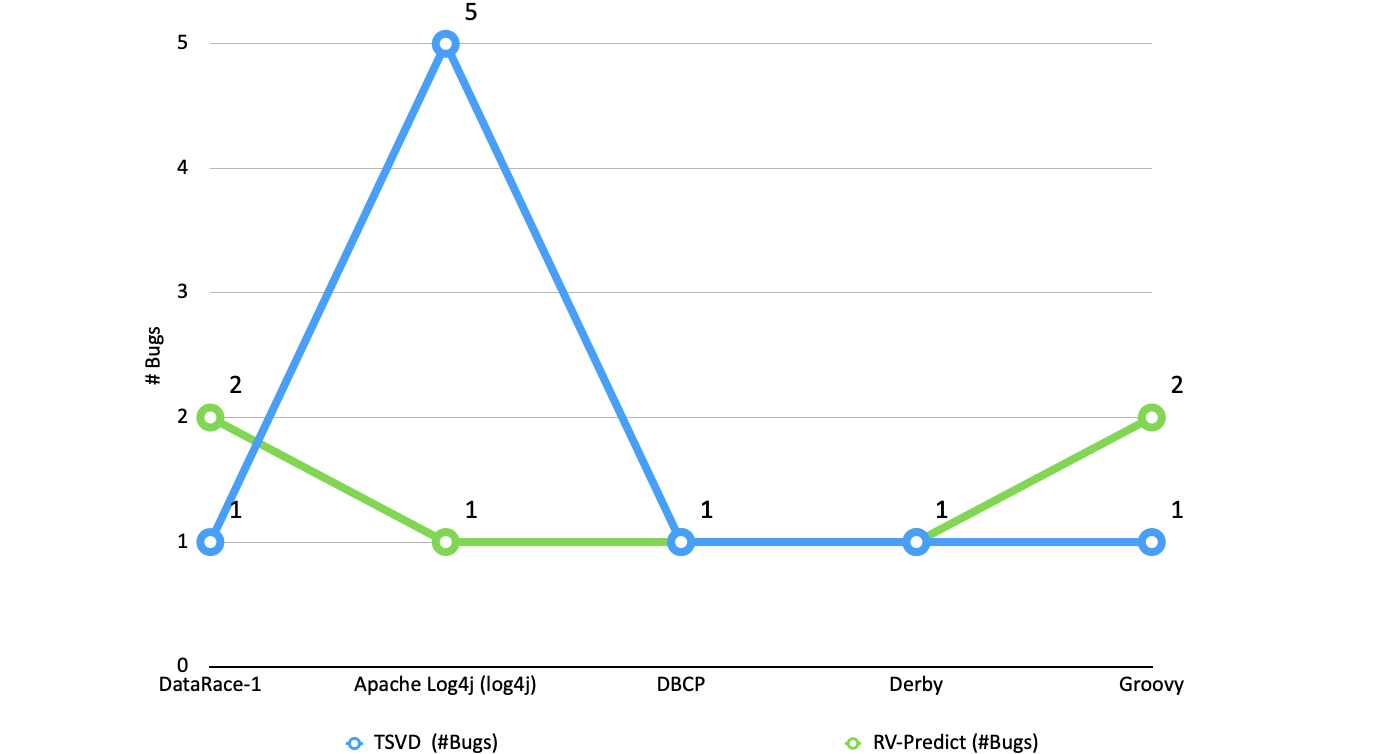
\includegraphics[width=0.5\textwidth]{images/graph.png}
	\label{fig:comparison}
	\caption{Result Comparison between Enhanced TSVD and RV-Predict}
\end{figure}


%\begin{table}
%	\centering
%	\caption{comparison with RV-Predict}
%	\label{table:comparison}
%	\begin{tabular}{|l|l|l|}
%		\hline
%		Project Name         & \begin{tabular}[c]{@{}l@{}}TSVD \\ (\#Bugs)\end{tabular} & \begin{tabular}[c]{@{}l@{}}RV-Predict \\ (\#Bugs)\end{tabular} \\ \hline
%			Apache Log4j (log4j) & 5             & 1                   \\ \hline
%			DBCP                 & 1             & 1                   \\ \hline
%			Derby                & 1             & 1                   \\ \hline
%			Groovy               & 1             & 2                   \\ \hline
%	\end{tabular}
%\end{table}

Overall our experiments suggest that our enhanced TSVD can detect concurrency related bugs more specifically data-race, which is one of the very time-demand problems. 

%\subsubsection{  }




%Just want to say that results for \Use{apache/hadoop_name} is
%\Use{apache/hadoop_result_num}.

%\subsection{RQ2: Second research question}
%\label{sec:eval:rq2}

%\input{tables/table.tex}
%\begin{table*}
	\centering
	\caption{the initial dataset}
	\label{table:dataset}
	\begin{tabular}{l|r|rr|r}
		\toprule
		\textbf{Id} & \multicolumn{1}{c|}{\textbf{project\_category}} & \multicolumn{1}{c}{\textbf{project\_name}} & \multicolumn{1}{c|}{\textbf{nums\_of\_lines}} & \multicolumn{1}{c}{\textbf{nums\_of\_tests}}\\
		\midrule
		\cline{1-5} \Use{Data-Race_project_id} & \multirow{2}{*}{toy project} & \Use{Data-Race_name} & \Use{Data-Race_nums_of_lines} & \Use{Data-Race_nums_of_tests}\\
		\Use{DataRace-Toy-Project2_project_id} &  & \Use{DataRace-Toy-Project2_name} & \Use{DataRace-Toy-Project2_nums_of_lines} & \Use{DataRace-Toy-Project2_nums_of_tests}\\
		\cline{1-5} \Use{Apache Log4j (log4j)_project_id} & \multirow{7}{*}{JaConTeBe} & \Use{Apache Log4j (log4j)_name} & \Use{Apache Log4j (log4j)_nums_of_lines} & \Use{Apache Log4j (log4j)_nums_of_tests}\\
		\Use{Apache Dbcp (dbcp)_project_id} &  & \Use{Apache Dbcp (dbcp)_name} & \Use{Apache Dbcp (dbcp)_nums_of_lines} & \Use{Apache Dbcp (dbcp)_nums_of_tests}\\
		\Use{Apache Derby (derby)_project_id} &  & \Use{Apache Derby (derby)_name} & \Use{Apache Derby (derby)_nums_of_lines} & \Use{Apache Derby (derby)_nums_of_tests}\\
		\Use{Apache Groovy (groovy)_project_id} &  & \Use{Apache Groovy (groovy)_name} & \Use{Apache Groovy (groovy)_nums_of_lines} & \Use{Apache Groovy (groovy)_nums_of_tests}\\
		\Use{OpenJdk (jdk-6, jdk-7)_project_id} &  & \Use{OpenJdk (jdk-6, jdk-7)_name} & \Use{OpenJdk (jdk-6, jdk-7)_nums_of_lines} & \Use{OpenJdk (jdk-6, jdk-7)_nums_of_tests}\\
		\Use{Apache Lucene (lucene)_project_id} &  & \Use{Apache Lucene (lucene)_name} & \Use{Apache Lucene (lucene)_nums_of_lines} & \Use{Apache Lucene (lucene)_nums_of_tests}\\
		\Use{Apache Pool (pool)_project_id} &  & \Use{Apache Pool (pool)_name} & \Use{Apache Pool (pool)_nums_of_lines} & \Use{Apache Pool (pool)_nums_of_tests}\\
		\cline{1-5} \Use{Java-WebSocket_project_id} & \multirow{22}{*}{github} & \Use{Java-WebSocket_name} & \Use{Java-WebSocket_nums_of_lines} & \Use{Java-WebSocket_nums_of_tests}\\
		\Use{macrozheng/mall_project_id} &  & \Use{macrozheng/mall_name} & \Use{macrozheng/mall_nums_of_lines} & \Use{macrozheng/mall_nums_of_tests}\\
		\Use{google/guava_project_id} &  & \Use{google/guava_name} & \Use{google/guava_nums_of_lines} & \Use{google/guava_nums_of_tests}\\
		\Use{eugenp/tutorials_project_id} &  & \Use{eugenp/tutorials_name} & \Use{eugenp/tutorials_nums_of_lines} & \Use{eugenp/tutorials_nums_of_tests}\\
		\Use{apolloconfig/apollo_project_id} &  & \Use{apolloconfig/apollo_name} & \Use{apolloconfig/apollo_nums_of_lines} & \Use{apolloconfig/apollo_nums_of_tests}\\
		\Use{alibaba/druid_project_id} &  & \Use{alibaba/druid_name} & \Use{alibaba/druid_nums_of_lines} & \Use{alibaba/druid_nums_of_tests}\\
		\Use{alibaba/fastjson_project_id} &  & \Use{alibaba/fastjson_name} & \Use{alibaba/fastjson_nums_of_lines} & \Use{alibaba/fastjson_nums_of_tests}\\
		\Use{xkcoding/spring-boot-demo_project_id} &  & \Use{xkcoding/spring-boot-demo_name} & \Use{xkcoding/spring-boot-demo_nums_of_lines} & \Use{xkcoding/spring-boot-demo_nums_of_tests}\\
		\Use{alibaba/easyexcel_project_id} &  & \Use{alibaba/easyexcel_name} & \Use{alibaba/easyexcel_nums_of_lines} & \Use{alibaba/easyexcel_nums_of_tests}\\
		\Use{alibaba/canal_project_id} &  & \Use{alibaba/canal_name} & \Use{alibaba/canal_nums_of_lines} & \Use{alibaba/canal_nums_of_tests}\\
		\Use{seata/seata_project_id} &  & \Use{seata/seata_name} & \Use{seata/seata_nums_of_lines} & \Use{seata/seata_nums_of_tests}\\
		\Use{xuxueli/xxl-job_project_id} &  & \Use{xuxueli/xxl-job_name} & \Use{xuxueli/xxl-job_nums_of_lines} & \Use{xuxueli/xxl-job_nums_of_tests}\\
		\Use{jenkinsci/jenkins_project_id} &  & \Use{jenkinsci/jenkins_name} & \Use{jenkinsci/jenkins_nums_of_lines} & \Use{jenkinsci/jenkins_nums_of_tests}\\
		\Use{alibaba/Sentinel_project_id} &  & \Use{alibaba/Sentinel_name} & \Use{alibaba/Sentinel_nums_of_lines} & \Use{alibaba/Sentinel_nums_of_tests}\\
		\Use{elunez/eladmin_project_id} &  & \Use{elunez/eladmin_name} & \Use{elunez/eladmin_nums_of_lines} & \Use{elunez/eladmin_nums_of_tests}\\
		\Use{linlinjava/litemall_project_id} &  & \Use{linlinjava/litemall_name} & \Use{linlinjava/litemall_nums_of_lines} & \Use{linlinjava/litemall_nums_of_tests}\\
		\Use{EnterpriseQualityCoding/FizzBuzzEnterpriseEdition_project_id} &  & \Use{EnterpriseQualityCoding/FizzBuzzEnterpriseEdition_name} & \Use{EnterpriseQualityCoding/FizzBuzzEnterpriseEdition_nums_of_lines} & \Use{EnterpriseQualityCoding/FizzBuzzEnterpriseEdition_nums_of_tests}\\
		\Use{openzipkin/zipkin_project_id} &  & \Use{openzipkin/zipkin_name} & \Use{openzipkin/zipkin_nums_of_lines} & \Use{openzipkin/zipkin_nums_of_tests}\\
		\Use{apache/shardingsphere_project_id} &  & \Use{apache/shardingsphere_name} & \Use{apache/shardingsphere_nums_of_lines} & \Use{apache/shardingsphere_nums_of_tests}\\
		\Use{JeffLi1993/springboot-learning-example_project_id} &  & \Use{JeffLi1993/springboot-learning-example_name} & \Use{JeffLi1993/springboot-learning-example_nums_of_lines} & \Use{JeffLi1993/springboot-learning-example_nums_of_tests}\\
		\Use{eclipse-vertx/vert.x_project_id} &  & \Use{eclipse-vertx/vert.x_name} & \Use{eclipse-vertx/vert.x_nums_of_lines} & \Use{eclipse-vertx/vert.x_nums_of_tests}\\
		\Use{YunaiV/SpringBoot-Labs_project_id} &  & \Use{YunaiV/SpringBoot-Labs_name} & \Use{YunaiV/SpringBoot-Labs_nums_of_lines} & \Use{YunaiV/SpringBoot-Labs_nums_of_tests}\\
		\midrule
		\bottomrule
	\end{tabular}
\end{table*}


%\begin{table*}
\centering
\caption{bugs found}
%\label{table:debug}
\resizebox{\textwidth}{!}{
\begin{tabular}{l|r|rr|r}
\toprule
\textbf{Project\_name} & \multicolumn{1}{c|}{\textbf{conflicting\_location}} & \multicolumn{1}{c}{\textbf{bugs}} & \multicolumn{1}{c|}{\textbf{lines}} & \multicolumn{1}{c}{\textbf{runs}}\\
\midrule
\Use{DataRace1_0_for_bug_name} & \Use{DataRace1_0_conflicting_location} & \Use{DataRace1_0_bug} & \Use{DataRace1_0_line} & \Use{DataRace1_0_run}\\
\Use{DataRace2_1_for_bug_name} & \Use{DataRace2_1_conflicting_location} & \Use{DataRace2_1_bug} & \Use{DataRace2_1_line} & \Use{DataRace2_1_run}\\
\Use{Apache Log4j (log4j)_2_for_bug_name} & \Use{Apache Log4j (log4j)_2_conflicting_location} & \Use{Apache Log4j (log4j)_2_bug} & \Use{Apache Log4j (log4j)_2_line} & \Use{Apache Log4j (log4j)_2_run}\\
\Use{Apache Log4j (log4j)_3_for_bug_name} & \Use{Apache Log4j (log4j)_3_conflicting_location} & \Use{Apache Log4j (log4j)_3_bug} & \Use{Apache Log4j (log4j)_3_line} & \Use{Apache Log4j (log4j)_3_run}\\
\Use{DBCP_4_for_bug_name} & \Use{DBCP_4_conflicting_location} & \Use{DBCP_4_bug} & \Use{DBCP_4_line} & \Use{DBCP_4_run}\\
\Use{Derby_5_for_bug_name} & \Use{Derby_5_conflicting_location} & \Use{Derby_5_bug} & \Use{Derby_5_line} & \Use{Derby_5_run}\\
\Use{Groovy_6_for_bug_name} & \Use{Groovy_6_conflicting_location} & \Use{Groovy_6_bug} & \Use{Groovy_6_line} & \Use{Groovy_6_run}\\
\Use{JeffLi1993/springboot-learning-example_7_for_bug_name} & \Use{JeffLi1993/springboot-learning-example_7_conflicting_location} & \Use{JeffLi1993/springboot-learning-example_7_bug} & \Use{JeffLi1993/springboot-learning-example_7_line} & \Use{JeffLi1993/springboot-learning-example_7_run}\\
\Use{xkcoding/spring-boot-demo_8_for_bug_name} & \Use{xkcoding/spring-boot-demo_8_conflicting_location} & \Use{xkcoding/spring-boot-demo_8_bug} & \Use{xkcoding/spring-boot-demo_8_line} & \Use{xkcoding/spring-boot-demo_8_run}\\
\midrule
\bottomrule
\end{tabular}}
\label{tbl:bug_found}
\end{table*}


%\begin{table*}
\centering
\caption{comparison with RV\_Predict}
\label{table:comparison}
\begin{tabular}{l|r|r|r}
\toprule
\textbf{Project\_name} & \multicolumn{1}{c|}{\textbf{\# TSVD}} & \multicolumn{1}{c}{\textbf{\# RV\_Predice}}\\
\midrule
\Use{Apache Log4j (log4j)_0_for_name} & \Use{Apache Log4j (log4j)_0_TSVD_bug} & \Use{Apache Log4j (log4j)_0_RV_bug}\\
\Use{DBCP_1_for_name} & \Use{DBCP_1_TSVD_bug} & \Use{DBCP_1_RV_bug}\\
\Use{Derby_2_for_name} & \Use{Derby_2_TSVD_bug} & \Use{Derby_2_RV_bug}\\
\Use{Groovy_3_for_name} & \Use{Groovy_3_TSVD_bug} & \Use{Groovy_3_RV_bug}\\
\midrule
\bottomrule
\end{tabular}
\end{table*}


%\begin{table*}
\centering
\caption{\TableCaption{}}
\label{table:tab}
\begin{tabular}{l|r}
\toprule
\textbf{Project} & \multicolumn{1}{c}{\textbf{\TableHeader{}}}\\
\midrule
\Use{macrozheng/mall,f2b823322e630794f61f3206430e12f01a359740,8.511650491,0_name} & \Use{macrozheng/mall,f2b823322e630794f61f3206430e12f01a359740,8.511650491,0_result_num}\\
\Use{google/guava,a2bbcc3bc2b4f94666d99a98a31445b8fbd1e152,602.938644089,0_name} & \Use{google/guava,a2bbcc3bc2b4f94666d99a98a31445b8fbd1e152,602.938644089,0_result_num}\\
\Use{eugenp/tutorials,18464bf799a6242582e7175f961a37d1463ce855,1.213039607,0_name} & \Use{eugenp/tutorials,18464bf799a6242582e7175f961a37d1463ce855,1.213039607,0_result_num}\\
\Use{apolloconfig/apollo,5ad5b410f0ff43111855d7bd76e047d08ab477b4,3280.048409263,0_name} & \Use{apolloconfig/apollo,5ad5b410f0ff43111855d7bd76e047d08ab477b4,3280.048409263,0_result_num}\\
\Use{alibaba/druid,98f6ea65ae08128829dadc788147e509b7876d82,37788.355126452,1_name} & \Use{alibaba/druid,98f6ea65ae08128829dadc788147e509b7876d82,37788.355126452,1_result_num}\\
\Use{alibaba/fastjson,869746101f6dd73b70d8a9c2b6dc59de4352519e,11.660334391,0_name} & \Use{alibaba/fastjson,869746101f6dd73b70d8a9c2b6dc59de4352519e,11.660334391,0_result_num}\\
\Use{xkcoding/spring-boot-demo,f10dc0a45be84e89acb48f6cf259620f52838b6e,43605.402173352,1_name} & \Use{xkcoding/spring-boot-demo,f10dc0a45be84e89acb48f6cf259620f52838b6e,43605.402173352,1_result_num}\\
\Use{alibaba/easyexcel,f8fd5f0427f04574c6d672615e8256c603e0b172,152.685562696,0_name} & \Use{alibaba/easyexcel,f8fd5f0427f04574c6d672615e8256c603e0b172,152.685562696,0_result_num}\\
\Use{alibaba/canal,b54bea5e3337c9597c427a53071d214ff04628d1,9324.229059803,0_name} & \Use{alibaba/canal,b54bea5e3337c9597c427a53071d214ff04628d1,9324.229059803,0_result_num}\\
\Use{seata/seata,6f877fafd0bc4ad2f4840e7940c93493f9aa45d5,8058.913255381,0_name} & \Use{seata/seata,6f877fafd0bc4ad2f4840e7940c93493f9aa45d5,8058.913255381,0_result_num}\\
\Use{xuxueli/xxl-job,9fe7aaa12e69ddb3cf99ee5681adbc32aa65ad54,2.662444141,0_name} & \Use{xuxueli/xxl-job,9fe7aaa12e69ddb3cf99ee5681adbc32aa65ad54,2.662444141,0_result_num}\\
\Use{jenkinsci/jenkins,cc30606c2706b4218acdfd5704fec37278a2cf25,75.748389700,0_name} & \Use{jenkinsci/jenkins,cc30606c2706b4218acdfd5704fec37278a2cf25,75.748389700,0_result_num}\\
\Use{alibaba/Sentinel,0a34fc4d11392f0587e7ba5bf2626f902b23c750,23.776244769,0_name} & \Use{alibaba/Sentinel,0a34fc4d11392f0587e7ba5bf2626f902b23c750,23.776244769,0_result_num}\\
\Use{elunez/eladmin,08f6c582112cdeaa785d79f04bbc90d4c0ca9b62,69042.975139933,0_name} & \Use{elunez/eladmin,08f6c582112cdeaa785d79f04bbc90d4c0ca9b62,69042.975139933,0_result_num}\\
\Use{linlinjava/litemall,7d79dfc68c36bd31e30c72acfdfd366f932bde0f,23,0_name} & \Use{linlinjava/litemall,7d79dfc68c36bd31e30c72acfdfd366f932bde0f,23,0_result_num}\\
\Use{EnterpriseQualityCoding/FizzBuzzEnterpriseEdition,4922c077c07a3744ae67ee8a932786f15bf57411,9.911529506,0_name} & \Use{EnterpriseQualityCoding/FizzBuzzEnterpriseEdition,4922c077c07a3744ae67ee8a932786f15bf57411,9.911529506,0_result_num}\\
\Use{openzipkin/zipkin,745fbad95878ed56588c8fb562ce0b2f9da17b4f,36757.205637363,0_name} & \Use{openzipkin/zipkin,745fbad95878ed56588c8fb562ce0b2f9da17b4f,36757.205637363,0_result_num}\\
\Use{apache/shardingsphere,011e12e18ed0c02b27ef23f7c46f0a99209446bb,86771.741120149,0_name} & \Use{apache/shardingsphere,011e12e18ed0c02b27ef23f7c46f0a99209446bb,86771.741120149,0_result_num}\\
\Use{JeffLi1993/springboot-learning-example,87692cb86fade44b2a368bf625abeaecb56709a6,1496.681491686,3_name} & \Use{JeffLi1993/springboot-learning-example,87692cb86fade44b2a368bf625abeaecb56709a6,1496.681491686,3_result_num}\\
\Use{eclipse-vertx/vert.x,3c494da0a4a854e52ee64f3571dc054d3d1d8ae3,10.763209883,0_name} & \Use{eclipse-vertx/vert.x,3c494da0a4a854e52ee64f3571dc054d3d1d8ae3,10.763209883,0_result_num}\\
\Use{YunaiV/SpringBoot-Labs,85c7322b9d1a225a4ba095f28a2b7f4b8f257da5,2.713523034,0_name} & \Use{YunaiV/SpringBoot-Labs,85c7322b9d1a225a4ba095f28a2b7f4b8f257da5,2.713523034,0_result_num}\\
\Use{xkcoding/spring-boot-demo,f10dc0a45be84e89acb48f6cf259620f52838b6e,65832.816014323,5_name} & \Use{xkcoding/spring-boot-demo,f10dc0a45be84e89acb48f6cf259620f52838b6e,65832.816014323,5_result_num}\\
\Use{alibaba/druid,98f6ea65ae08128829dadc788147e509b7876d82_name} & \Use{alibaba/druid,98f6ea65ae08128829dadc788147e509b7876d82_result_num}\\
\midrule
Overall & \Use{overall_result_num}\\
\bottomrule
\end{tabular}
\end{table*}


%Table~\ref{table:tab} shows our results.




